\documentclass[a4paper]{article}
\usepackage{tikz}
\usepackage[a4paper,margin=0.5cm]{geometry}
\usepackage{textcomp}

\newcommand{\sometext}{
sol\textbullet{}ami\textbullet{}x testlabel\textbar etiquette de test\\
zutat 1 80\% (vom Hof), zutat 2 20\% (EU)\textbar ingredient 1 80\% (de la ferme), ingredient 2 20\% (origin) \\
abgefüllt\textbar mise en pot du@example.org\\
mindestens haltbar bis\textbar à consommer avant le (datum)\\
weiterer infos\textbar info additionelle\\
verein sol\textbullet{}ami\textbullet{}x, Alexander-Moser-Strasse 28, 2503 Biel/Bienne
}

\newcommand{\labelw}{10.5cm}
\newcommand{\labelh}{3.0cm}
\newcommand{\textw}{\dimexpr\labelw-0.2cm\relax}

% spacing labelh + cm margin
\newcommand{\spaceh}{\dimexpr\labelh+0.2cm\relax}
% vertical spacing: 0.5 * \labelh
\newcommand{\labelc}{\dimexpr\labelh/2\relax}


\begin{document}

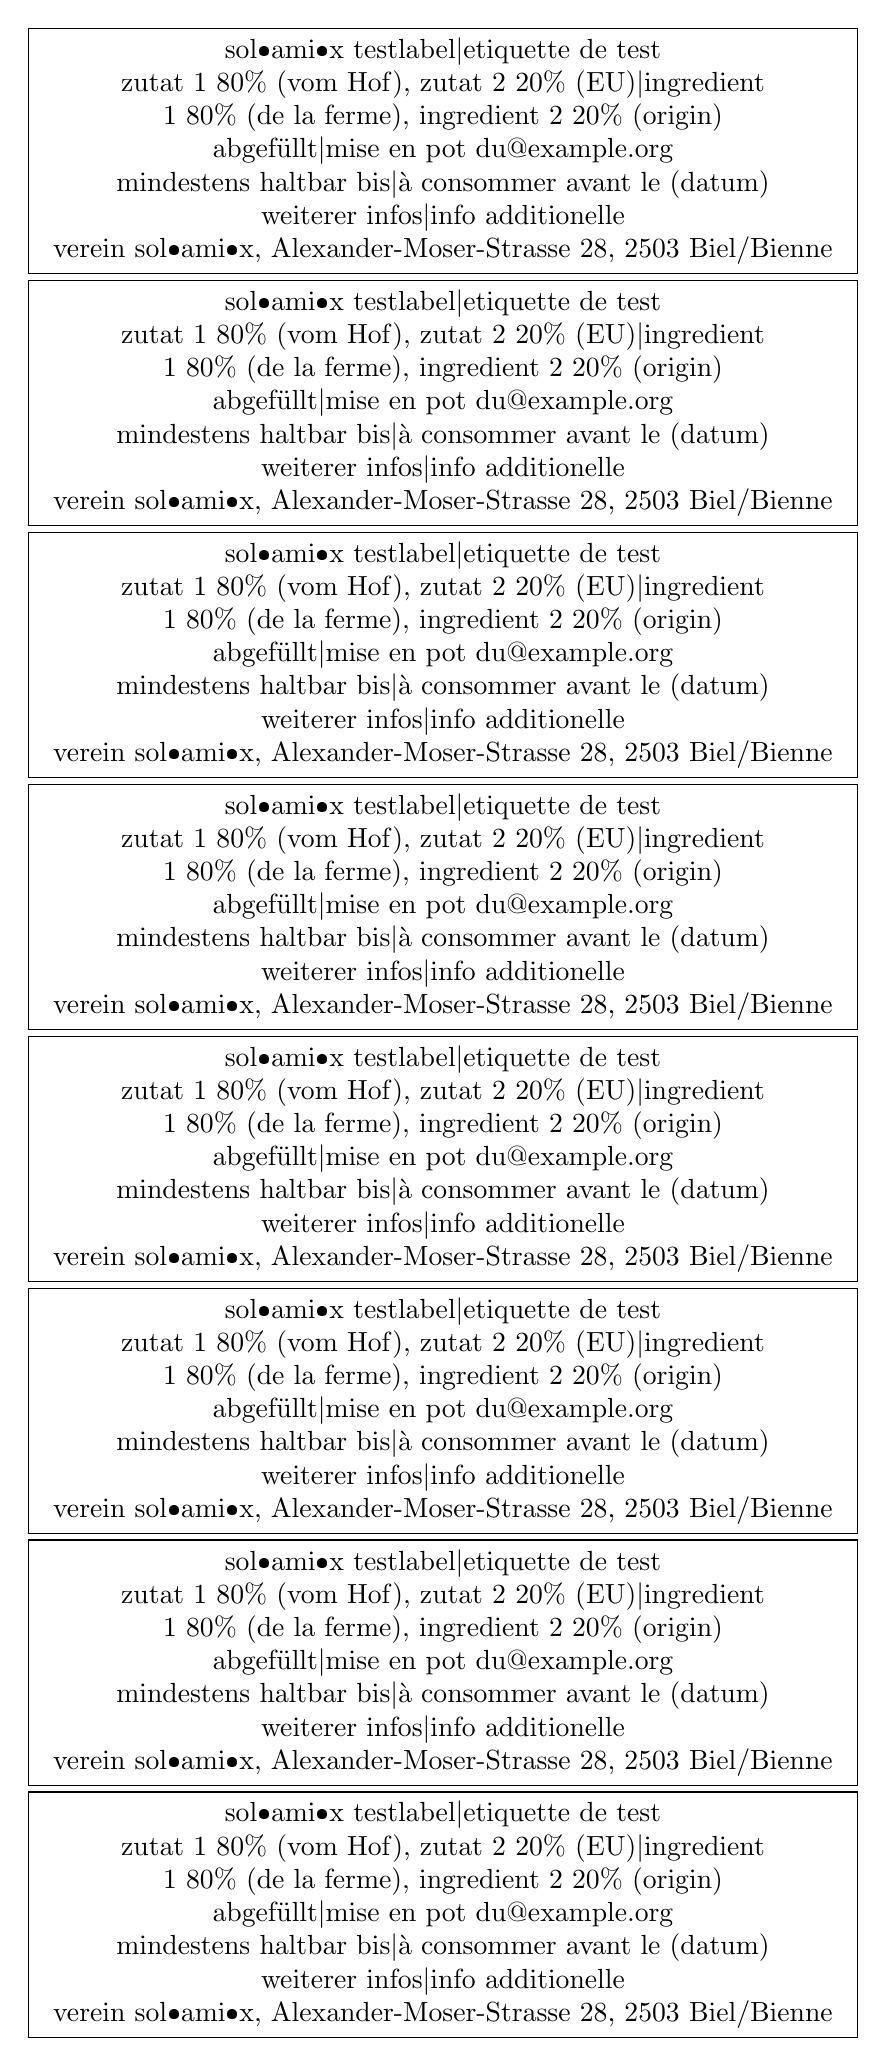
\begin{tikzpicture}
    \foreach \j in {0,...,7} {
        \node[rectangle, minimum width=\labelw, minimum height=\labelh, draw, text width=\textw, align=center] at (3cm, \spaceh*\j+\labelc) {\sometext};
    }
\end{tikzpicture}

\end{document}
